\documentclass[tikz, border=5pt]{standalone}

\begin{document}

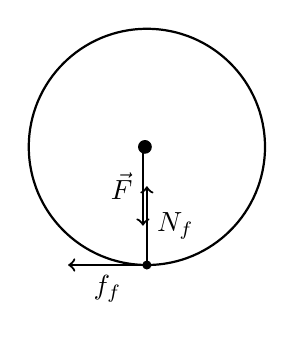
\begin{tikzpicture}

    %% FBD of Front wheel

    % Front wheel
    \draw[thick] (0,0) circle(1.5);
    \draw[fill] (-0.025,0) circle(0.08);

    % Normal force
    \draw[->, thick] (0,-1.5) -- (0,-0.5) node[midway,right] {$N_f$};
    \draw[fill] (0,-1.5) circle(0.05);

    % Applied force on the pedal
    \draw[->, thick] (-0.05,0) -- (-0.05,-1) node[midway,left] {$\vec{F}$};

    % Frictional force
    \draw[->, thick] (0,-1.5) -- (-1,-1.5) node[midway,below] {$f_f$};

\end{tikzpicture}

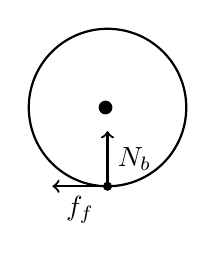
\begin{tikzpicture}

    %% FBD of Back wheel

    % Back wheel
    \draw[thick] (0,0) circle(1);
    \draw[fill] (-0.025,0) circle(0.08);

    % Normal force
    \draw[->, thick] (0,-1) -- (0,-0.3) node[midway,right] {$N_b$};
    \draw[fill] (0,-1) circle(0.05);

    % Frictional force
    \draw[->, thick] (0,-1) -- (-0.7,-1) node[midway,below] {$f_f$};

\end{tikzpicture}

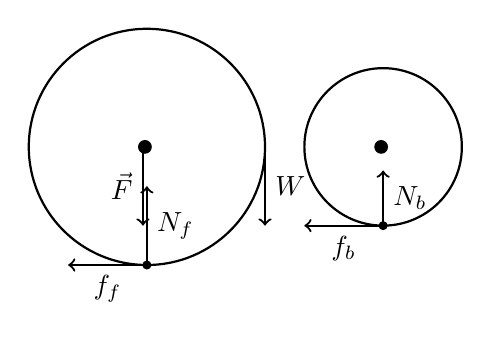
\begin{tikzpicture}

    %% FBD of Entire Bicycle

    % Front wheel
    \draw[thick] (0,0) circle(1.5);
    \draw[fill] (-0.025,0) circle(0.08);

    % Back wheel
    \draw[thick] (3,0) circle(1);
    \draw[fill] (3-0.025,0) circle(0.08);

    % Normal force on front wheel
    \draw[->, thick] (0,-1.5) -- (0,-0.5) node[midway,right] {$N_f$};
    \draw[fill] (0,-1.5) circle(0.05);

    % Normal force on back wheel
    \draw[->, thick] (3,-1) -- (3,-0.3) node[midway,right] {$N_b$};
    \draw[fill] (3,-1) circle(0.05);

    % Applied force on the pedal
    \draw[->, thick] (-0.05,0) -- (-0.05,-1) node[midway,left] {$\vec{F}$};

    % Frictional force on front wheel
    \draw[->, thick] (0,-1.5) -- (-1,-1.5) node[midway,below] {$f_f$};

    % Frictional force on back wheel
    \draw[->, thick] (3,-1) -- (2,-1) node[midway,below] {$f_b$};

    % Weight of the bicycle
    \draw[->, thick] (1.5,0) -- (1.5,-1) node[midway,right] {$W$};

\end{tikzpicture}

\end{document}
